%!TeX spellcheck = fr_FR
\documentclass[a4paper, 12pt]{article}
\usepackage[top = 1.6cm, left = 2cm, right = 2cm ]{geometry}
\usepackage[pdftex]{graphicx}
\usepackage{soulutf8}
\usepackage{amsmath}
\usepackage{amssymb}
\usepackage{tikz}
\usepackage[utf8]{inputenc}
\usepackage{longtable}
\usepackage[T1]{fontenc}
\usepackage{epigraph}
\usepackage{fancyhdr}
\usepackage{float}
\usepackage{subfig}
\usepackage{xcolor}
\usepackage{eurosym}
\usepackage{calc}
\usepackage{multirow} 
%
%
%%%%% Custom commands
%
%
\def\changemargin#1#2{\list{}{\rightmargin#2\leftmargin#1}\item[]}
\let\endchangemargin=\endlist 
%
\newcommand{\newlinealinea}{
~\\ \hspace*{0.5cm}}
%
\newcommand{\alinea}{
\hspace*{0.5cm}}
%
\newcommand{\alinealong}{
\hspace*{1.1cm}}
%
\newcommand{\alignparagraph}{
\hspace*{0.6cm}}
%
\newcommand{\red}[1]{
	\textcolor{red}{#1}}
%
\newcommand{\green}[1]{
	\textcolor{green}{#1}}
%
\newcommand{\point}{$\bullet\ $}
%
\makeatletter
	\newcommand*{\whiten}[1]{\llap{\textcolor{white}{{\the\SOUL@token}}\hspace{#1pt}}}
	\newcommand{\myul}[1]{
		\underline{\smash{#1}}
	}
\makeatother
%
\setlength{\fboxsep}{2pt}
%
\DeclareMathOperator*{\argmax}{\arg\!\max}
%
%
%%%%% Custom text
%
%
\makeatletter
\@addtoreset{section}{part}
\makeatother  
\renewcommand\partname{Partie} 
%
\renewcommand*\sfdefault{phv}
\renewcommand*\rmdefault{ppl}
%
\renewcommand\epigraphflush{flushright}
\renewcommand\epigraphsize{\normalsize}
\setlength\epigraphwidth{0.7\textwidth}
%
\definecolor{titlepagecolor}{cmyk}{0.24,0.92,0.78,0.25}
\definecolor{red}{cmyk}{0, 0.91, 0.91, 0.20}
%
\DeclareFixedFont{\titlefont}{T1}{phv}{\seriesdefault}{n}{0.375in}
%
%
%%%%% Header
%
%
\pagestyle{fancy}
\lhead{Anthony Rouneau}
\rhead{MAB2 Sciences Informatiques}
\cfoot{\thepage}
%
%
%%%%% Title page. The following code is borrowed from: 
%%%%%       http://tex.stackexchange.com/a/86310/10898
%
%
\newcommand\titlepagedecoration{%
\begin{tikzpicture}[remember picture,overlay,shorten >= -10pt]

\coordinate (aux1) at ([yshift=-70pt]current page.north east);
\coordinate (aux2) at ([yshift=-460pt]current page.north east);
\coordinate (aux3) at ([xshift=-6cm]current page.north east);
\coordinate (aux4) at ([yshift=-150pt]current page.north east);

\begin{scope}[titlepagecolor!40,line width=12pt,rounded corners=12pt]
\draw
  (aux1) -- coordinate (a)
  ++(225:5) --
  ++(-45:5.1) coordinate (b);
\draw[shorten <= -10pt]
  (aux3) --
  (a) --
  (aux1);
\draw[opacity=0.6,titlepagecolor,shorten <= -10pt]
  (b) --
  ++(225:2.2) --
  ++(-45:2.2);
\end{scope}
\draw[titlepagecolor,line width=8pt,rounded corners=8pt,shorten <= -10pt]
  (aux4) --
  ++(225:0.8) --
  ++(-45:0.8);
\begin{scope}[titlepagecolor!70,line width=6pt,rounded corners=8pt]
\draw[shorten <= -10pt]
  (aux2) --
  ++(225:3) coordinate[pos=0.45] (c) --
  ++(-45:3.1);
\draw
  (aux2) --
  (c) --
  ++(135:2.5) --
  ++(45:2.5) --
  ++(-45:2.5) coordinate[pos=0.3] (d);   
\draw 
  (d) -- +(45:1);
\end{scope}
\end{tikzpicture}%
}
%
\begin{document}
	\begin{titlepage}
	%
	\noindent
	%
	\newgeometry{bottom = 2cm, top = 2.5cm}
	\begin{center}
		
\includegraphics[scale=1.2]{Images/UMONS}\\
			\vspace*{0.3cm}
		
\includegraphics[scale=0.23]{Images/FS_Logo}\\
			\vspace*{2.5cm}
		%
		\titlefont Aide multicritère à la décision\\~\\ {\huge Résumé} \par
		%
	\end{center}
	\vspace*{3cm}
	\hfill
	%
	\begin{minipage}{0.18\linewidth}
		\begin{flushright}
			\rule{0.5pt}{75pt}
		\end{flushright}
	\end{minipage}
	%
	\begin{minipage}{0.8\linewidth}
		\begin{flushleft}
			\textsf{\textbf{Résumé réalisé par:}} Anthony Rouneau\\
			\textsf{\textbf{Section:}} 2$^{\text{\`eme}}$ Bloc Master en 
				Sciences Informatiques\\
			\textsf{\textbf{Images:}} Proviennent du cours de M. Pirlot.\\
		\end{flushleft}
	\end{minipage}
	%
	\vspace*{\fill}                                                             
	%
	\begin{center}
		Faculté des Sciences $\bullet$ Université de Mons $\bullet$ 
		Place du Parc 20 $\bullet$ B-7000 Mons
	\end{center}
	%
	\titlepagedecoration
	%
\end{titlepage}
%
%
%%%% Tables des matières
%
%
\newgeometry{top = 3cm, left = 2cm, right = 2cm, bottom=2.5cm}
%
\tableofcontents
%
\newpage
%
\section{Introduction}
	\subsection{Types de problèmes}
		\begin{itemize}
			\setlength\itemsep{0cm}
			\item \red{Make or buy} -- Décider si on achète à un tiers ou si on produit nous même. Si on produit ça coute plus cher
				mais ça nécessite l'infrastructure et les machines.
			\item \red{Management} -- Définir un ordre de priorité dans les projets internes.
			\item \red{Choix d'équipement} -- Retourne un objet.
			\item \red{Choix de candidats} -- Retourne un rangement parmi les candidats.
			\item \red{Classement de réponse à un appel d'offre} -- Retourne un tri en paquet.
			\item \red{\'Elections par votes} -- Les critères sont définis par les votants.
			\item \red{Trouver localisation optimale} -- Problème d'optimisation.
			\item \red{Gestion de portefeuille} -- Objectif : optimisation globale.
		\end{itemize}
	%
	\subsection{Problème de décision}
		\alinea Un problème de décision doit rester \hl{subjectif}. En effet, on doit respecter les préférences des parties 
			prenantes. Voici quelques \hl{mots de vocabulaire} : 
			\begin{itemize}
				\setlength\itemsep{0cm}
				\item \red{Décideur(s)} -- Responsable(s) de la décision.
				\item \red{Parties prenantes} -- personnes ayant un intérêt dans la décision.
				\begin{itemize}
					\setlength\itemsep{0cm}
					\item Peuvent ajouter des contraintes.
					\item Peuvent montrer de la résistance dans la prise de décision.
					\item Peuvent ajouter des informations utiles pour la prise de décision.
				\end{itemize}
				\item \red{Problématique} -- Choisir, ranger, trier, ...
				\item \red{Les actions ou alternatives} -- Les choix disponibles.
				\item \red{Les critères} -- Les qualités qui vont affecter le choix. Si les critères sont bien fixés, 
					le choix guidé par l'aide à la décision doit correspondre avec un choix idéal pour le décideur.
 			\end{itemize}
		%
		Il y a \hl{deux phases} principales dans la résolution d'un tel problème : 
			\begin{itemize}
				\setlength\itemsep{0cm}
				\item \red{Structuration} -- Définition des étapes de résolution.
				\item \red{Agrégation} -- \'Etablissement d'un modèle de préférence, validation des paramètres, ...
			\end{itemize}
		%
		Deux \hl{méthodes principales} peuvent être utilisée pour établir un classement dans les alternatives : 
			\begin{itemize}
				\setlength\itemsep{0cm}
				\item \red{Synthétique} -- Classement général, établi en fonction des critères.
				\item \red{Comparaison par pair} -- On compare les alternatives deux à deux selon les critères.
			\end{itemize}
		Dans le cas de \hl{critères discrets}, des problèmes mathématiques peuvent survenir. En effet si on classe des
			critères avec un entier entre 1 et 5, 2 ne vaut pas toujours le double de 1 (Comme si on notait A, B, C, D, ...).
			Malgré tout, on va considérer que 2 est le double de 1 dans les calculs.
			On peut se retrouver alors avec des \hl{échelles et des unités tout à fait hétérogènes}.
		%
	%
	\subsection{Dominance}
		\alinea On dit que $A$ \red{\hl{domine}} $B$ si l'objet $A$ obtient de \hl{meilleurs résultats sur tous les critères} 
			par rapport à l'objet $B$. Si le modèle est bon, on ne devrait alors \hl{jamais sélectionner $B$} dans la procédure de 
			décision.
		%
	%
%
\section{Critique de la somme pondérée}
	\subsection{Super-critère par somme pondérée}
		\alinea On parle de \red{super-critère par somme pondérée} pour un re-codage d'un critère existant en prenant en compte
			le poids accordé à ce critère. \hl{Ce re-codage $u$ vaut ceci} :
			$$ u(a) = \sum\limits_{i=1}^{n} k_i g_i (a)\text{, avec } a \text{ une des alternatives} $$
			$$ \text{avec } n \text{ le nombre de critères}$$			
			$$ \text{avec } g_i \text{ l'évaluation du critère } i $$
			$$ \text{avec } k_i \text{ le poids accordé au critère } i \text{, \hl{négatif si le critère est à minimiser}}$$
		%
		\alinea Le principe est donc de re-coder de cette manière toutes les alternatives afin de donner un \hl{"score" pondéré}
			à chacune d'elle. Ensuite, on peut comparer les alternatives entre elles selon leur super-critère : 
			$$ a \succsim b \Leftrightarrow u(a) \geqslant u(b) \Leftrightarrow \sum\limits_{i=1}^{n} k_i (g_i (a) - g_i (b)) \geqslant 0$$
		%
	%
	\subsection{Normalisation}
		\alinea Il existe \hl{plusieurs manières de normaliser}. \hl{Selon la méthode utilisée et selon les alternatives} prises dans la
			normalisation, le résultat de la prise de décision peut être différente. 
			\paragraph{Normaliser en fonction de la meilleures alternative}
				$$ g_i'(a) = \frac{g_i(a)}{\max g_i} $$
			%
			\paragraph{Normaliser pour que le min vaille 0 et le max vaille 1}
				$$ g_i'(a) = \frac{g_i(a) - \min g_i}{\max g_i - \min g_i} $$
			%
			\paragraph{Normaliser au sens statistique}
				$$ g_i'(a) = \frac{g_i(a) - \mu_{g_i}}{\sigma_{g_i}} $$
			%
		%
	%
	\subsection{Poids vs. taux de change}
		\alinea Le poids des critères ne représentent pas leur importance. Ce sont des \hl{taux de substitution}.
			\hl{Un désavantage de $k_i$ unités sur le critère j peut être compensé par un avantage de $k_j$ unités sur le critère i}.
			En effet, c'est pour garder l'importance d'un critère que l'on va adapter le poids.
			Par exemple, si on parlait de critères temporels et que les secondes avec un poids $k_s$, on accorderait un poids
			valant $k_s \cdot 60$ aux minutes afin que les minutes gardent leur importance, et $k_s \cdot 3600$ aux heures.
		%
	%
	\subsection{Préférence non-linéaire}
		\alinea En pratique, \hl{il arrive souvent que les préférences ne soient pas linéaires}. Exemple : on aimerait bien plus trouver
			une voiture entre 15000 et 20000 euros qu'entre 20000 et 30000. On va donc accorder plus d'importance aux voitures se 
			trouvant dans le premier intervalle. La somme pondérée \hl{ne permet pas d'exprimer des préférences non-linéaires}.
			En pratique, il faudra \hl{re-coder le super-critère} (pas celui de la somme pondérée) pour qu'il soit non-linéaire.
		%
	%
	\subsection{Indépendance préférentielle}
		\alinea La somme pondérée raisonne selon "ceteris paribus", qui veut dire "toutes choses restant égales par ailleurs". 
			\hl{\c Ca veut dire qu'en cas d'égalité entre plusieurs critères, ce sont les critères inégaux qui influenceront le choix.}
			\c Ca veut dire également que les \hl{préférences doivent être indépendantes} afin d'être utilisées dans une somme pondérées.
			Ce raisonnement n'est pas toujours pertinent. Prenons comme exemple un problème dans lequel on doit obtenir un ordre de
			préférence entre frite/pâtes (premier critère) et mayo/bolo (deuxième critère). soit $g_1(\text{frites}) = 0.4$, 
			$g_1(\text{pates}) = 0.7$, $g_2(\text{mayo}) = 0.6$ et $g_2(\text{bolo}) = 0.5$. On se retrouve alors avec
			$\text{frites mayo} > \text{frites bolo}$, ce qui semble correct, mais par contre, on a que 
			$\text{pates mayo} > \text{pates bolo}$, ce qui ne fera pas plaisir aux parties prenantes. Une solution serait de 
			\hl{regrouper les deux critères en un seul, car ils sont dépendants}.
		%
	%
	\subsection{\'Ecarts minimes}
		\alinea Même si il y a seulement une différence d'un centième entre deux alternatives, la somme pondérée va trancher.
			il faudrait donc faire \hl{une analyse de sensibilité}, c'est-à-dire faire varier les valeurs des poids et des évaluations
			pour voir si le même résultat en ressort.
		%
	%
	\subsection{Résumé}
		\begin{center}
			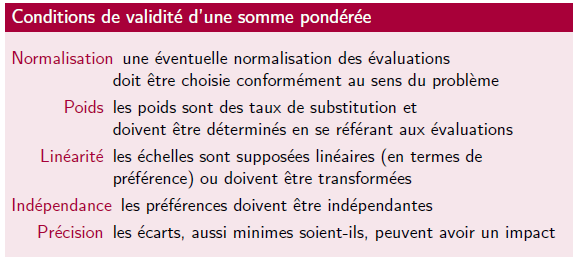
\includegraphics[width=5in]{Images/somme}
		\end{center}
	%
%
\section{Fonctions de valeur additive}
	\alinea Le principe ici est de calculer le \hl{super-critère des alternatives selon une somme de fonctions de re-codage}.
		On va supposer que chaque critère a sa propre fonction de re-codage.
		$$ u(a) = \sum\limits^{n}_{i=1} u_i(g_i(a)) $$
		ou encore, si on accorde des poids aux critères : 
		$$ u'(a) = \sum\limits^{n}_{i=1} k_i \cdot u_i'(g_i(a)) $$
		\begin{center}
		avec $u_i'(g_i, \min) = 0$, $u_i'(g_i, \max)$ et $\sum\limits^{n}_{i=1} k_i = 1$
		\end{center}
	%
	\subsection{Méthodes directes}
		\subsubsection{Jugements d'indifférence}
			\alinea Le principe ici est de demander aux parties prenantes d'\hl{estimer des valeurs pour lesquelles deux alternatives
				seraient indifférentes (équivalentes)}. Pour ce faire, on va avoir besoin d'un \hl{critère de base}, pour lequel
				on prendra un \hl{intervalle de valeur}. On part de la meilleure (resp. la moins bonne) valeur de cet intervalle et 
				d'une valeur marginale pour le critère à évaluer. On va ensuite à chercher une valeur pour le critère à évaluer tel 
				que l'alternative ayant	cette valeur et la moins bonne (resp. la meilleure) valeur pour le critère de base soit 
				indifférente à la première. Soit deux critères à minimiser : le prix et le temps d'accélération, voici un \hl{exemple} 
				de jugement d'indifférence :\\
				\begin{minipage}{0.49\textwidth}
					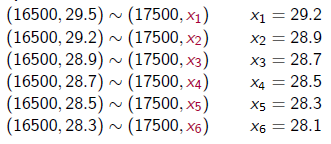
\includegraphics[width=\textwidth]{Images/indifference} 
				\end{minipage}\hfill
				\begin{minipage}{0.5\textwidth}
					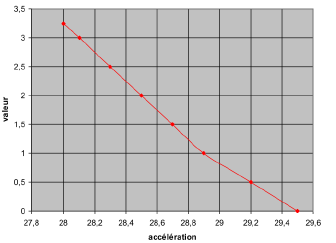
\includegraphics[width=\textwidth]{Images/indifference2}
				\end{minipage}~\\~\\~\\
			%
			\alinea Il ne manque plus qu'à \hl{normaliser la courbe} pour que la valeur soit comprise entre 0 et 1 (ou 0 et 100). 
				Il est alors simple de \hl{calculer les taux de substitution} (poids) :
				$$ \frac{k2}{k1} = \frac{u_1'(16500) - u_1'(17500)}{u_2'(29.2) - u_2'(29.5)} $$
			\alinea On fait pareil avec tous les critères (toujours en fonction du critère 1), et on finit par choisir $k_1$
				pour que l'équation $\sum\limits^{n}_{i=1} k_i = 1$ soit respectée.\\
			%
			~\\
			%
			\alinea En résumé, la technique est bonne mais présente quelques inconvénients :
				\begin{center}
					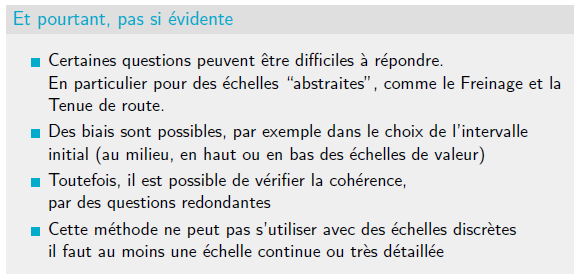
\includegraphics[width=5in]{Images/indifference3}
				\end{center}
			%
		%
		\subsubsection{Direct rating}
			\paragraph{SMART}
				\alinea Cette technique est très simple : on \hl{prend deux valeurs extrêmes}, et on leur attribue une valeur 
					d'utilité (pour $u$) : 0 pour la moins bonne, et 100 pour la meilleure. On va ensuite \hl{interroger le 
					décideur pour trouver les évaluations intermédiaires}. \\
				%
				\begin{minipage}{0.33\textwidth}
					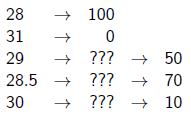
\includegraphics[width=\textwidth]{Images/smart1}
				\end{minipage}\hfill
				\begin{minipage}{0.575\textwidth}
					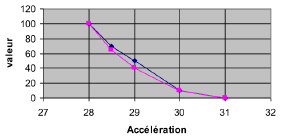
\includegraphics[width=\textwidth]{Images/smart2}
				\end{minipage}~\\~\\~\\
				%
				\alinea Une fois qu'on a effectué cette partie pour tous les critères, \hl{on donne 10 points (poids) au critère le moins
					important}, et on se base dessus pour assigner des poids aux autres critères. Il reste ensuite à normaliser
					les poids pour qu'ils somment à 1.
				%
			%
			\paragraph{Swing Weighting}
				\alinea Le principe ici est de faire une évaluations des alternatives. On part de la \hl{pire alternative possible},
					ce sera la référence. Ensuite, \hl{on demande au décideur quel premier critère permettrait d'améliorer cette
					alternative}, puis quel second critère améliorerait l'alternative, etc... On obtiendra donc un ordre d'importance 
					parmi les critères. Il suffit ensuite de pondérer ces critères selon l'ordre choisi, tout en respectant les 
					contraintes précédentes (poids somment à 1, ...).
				%
			%
		%
	%
	\subsection{Fonction de valeur additive (UTA)}
		\alinea Le but ici est de fournir une méthode \hl{automatisée} pour trouver la fonction de re-codage ainsi que le poids de 
			chaque critère. Pour trouver des fonctions de re-codage non-linéaires, on va donner une fonction linéaire par morceaux.
			Ces morceaux étant séparés par des points de cassure.
		%
		\begin{center}
			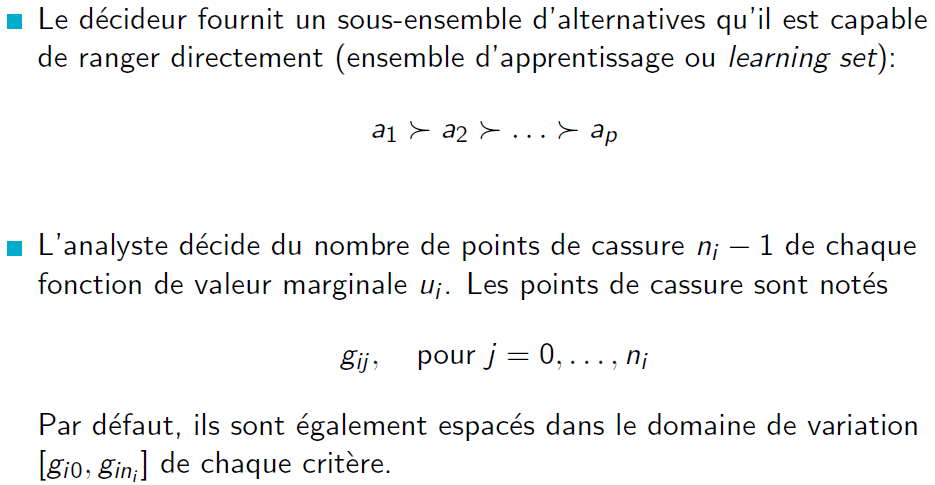
\includegraphics[width=5in]{Images/UTA0}
		\end{center}
		%
		\alinea L'apprentissage se fait ensuite selon un programme linéaire qui va chercher à \hl{maximiser l'écart entre les alternatives
			sélectionnées}.	Pour ce faire, l'apprentissage va chercher la position de ces points de cassure.
		%
		\begin{center}
			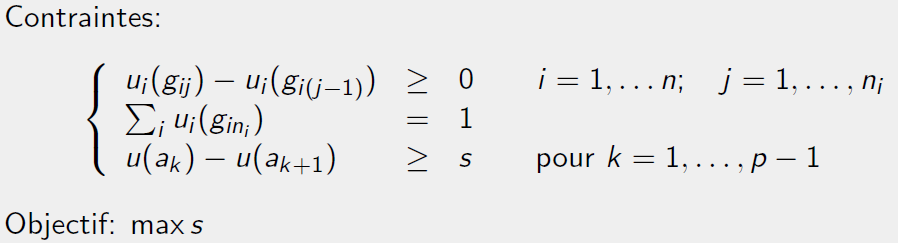
\includegraphics[width=4in]{Images/UTA1}
		\end{center}
		%
		\alinea Cependant, avec cette formulation, il est\hl{ possible qu'on ne trouve pas de solution} avec le nombre de points de cassure
			choisis et/ou les alternatives choisies. Pour résoudre ce problème, on va \hl{ajouter des pénalités} qui feront
			en sorte qu'il existe toujours une solution. Ces pénalités sont à minimiser, et dans l'idéal restent à 0 (ce qui veut
			dire qu'il n'y a pas besoin de pénalités pour que ça fonctionne).
		%
		\begin{center}
			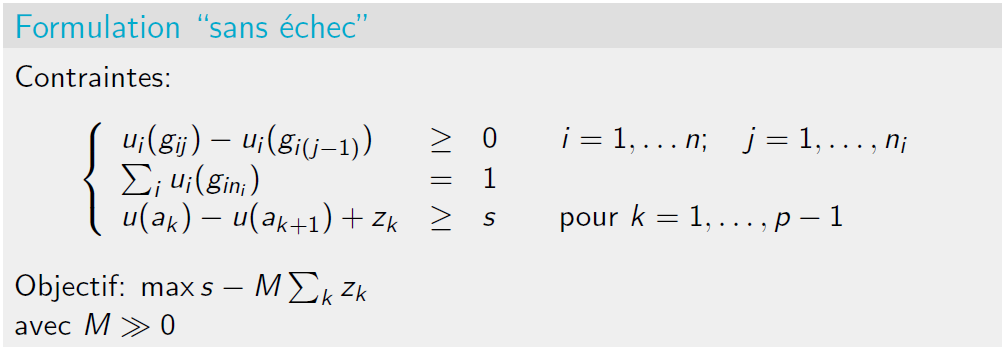
\includegraphics[width=4.5in]{Images/UTA2}
		\end{center}
		%
		\subsubsection{Théorème de représentation}
			\alinea Les préférences du décideur doivent \hl{respecter une liste de contraintes} afin de pouvoir être représentée par une 
				fonction de valeur additive. Si elle ne correspondent pas aux conditions suivantes, il faut choisir un autre modèle de 
				représentation.
			%
			\begin{center}
				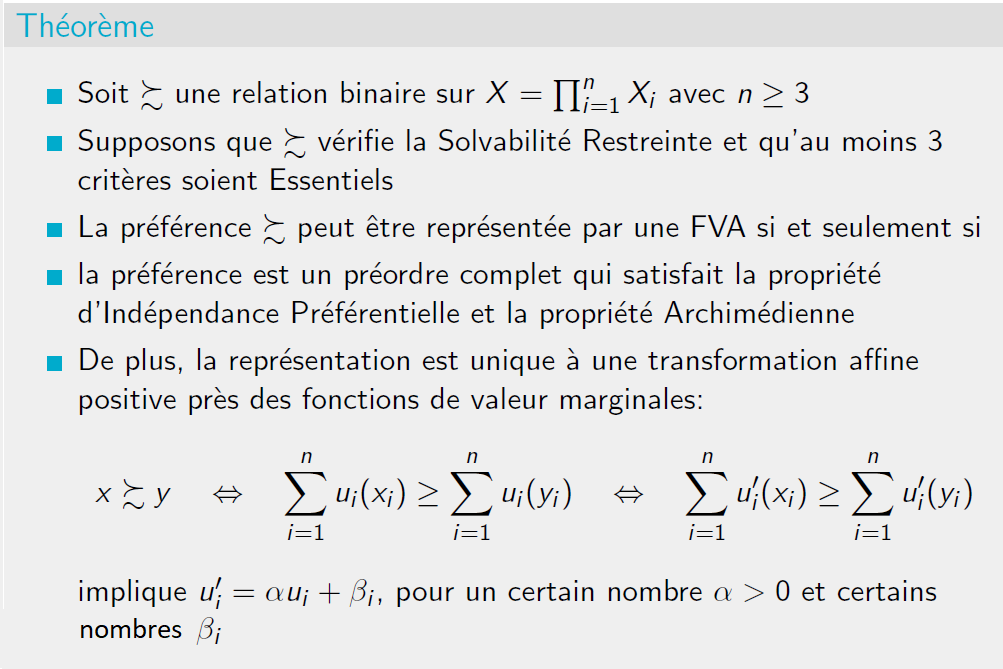
\includegraphics[width=4.5in]{Images/FVA}
			\end{center}
			%
			\begin{center}
				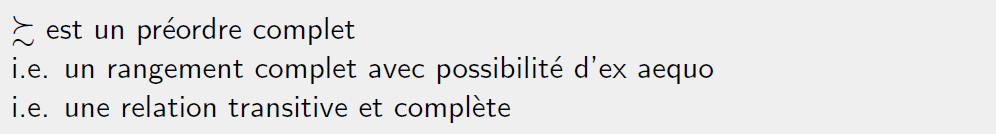
\includegraphics[width=4.5in]{Images/preordre}
			\end{center}
			%			
			\begin{center}
				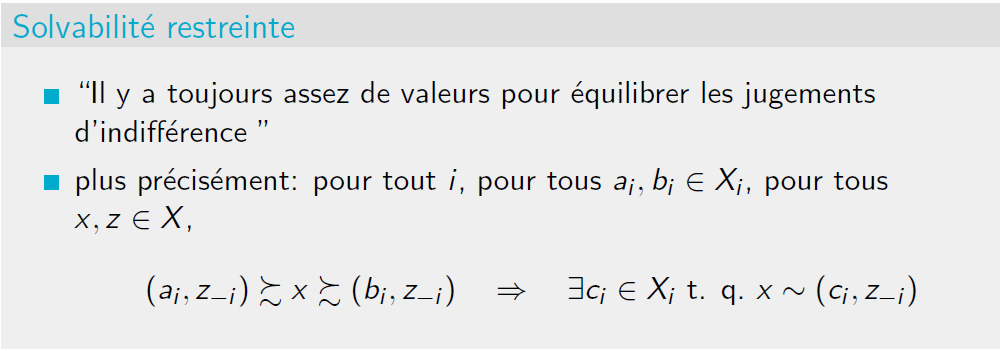
\includegraphics[width=4.5in]{Images/solvabilite_restreinte}
			\end{center}
			%
			\begin{center}
				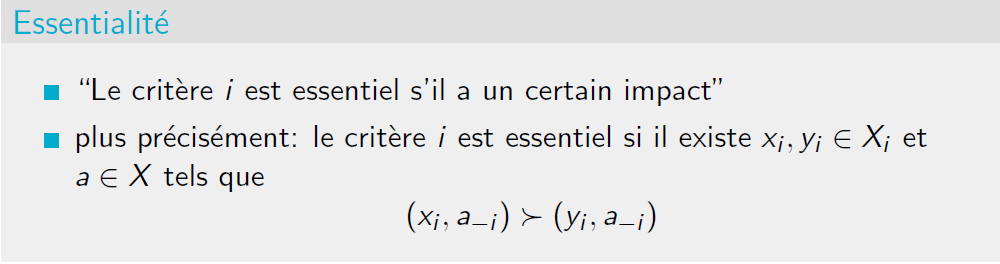
\includegraphics[width=4.5in]{Images/essentiel}
			\end{center}
			%
			\begin{center}
				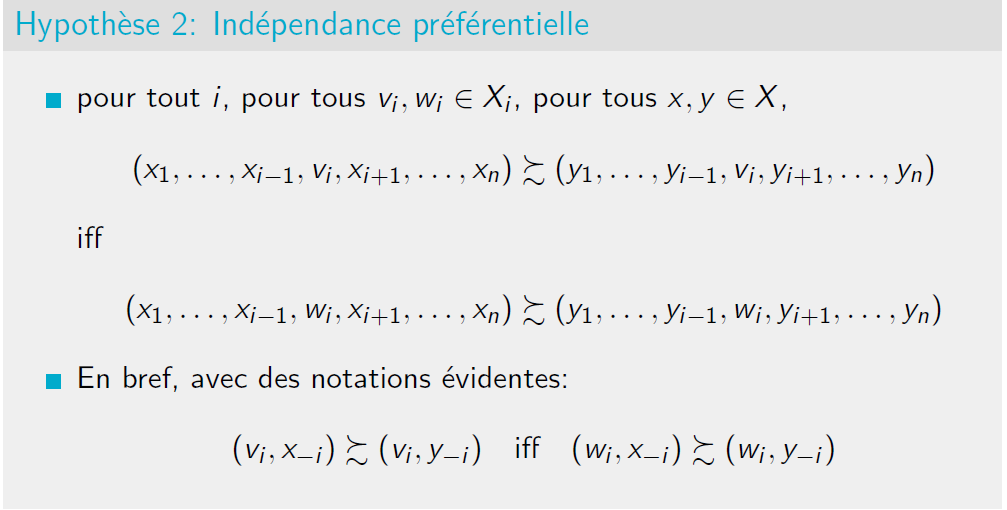
\includegraphics[width=4.5in]{Images/independance}
			\end{center}
			%
			\begin{center}
				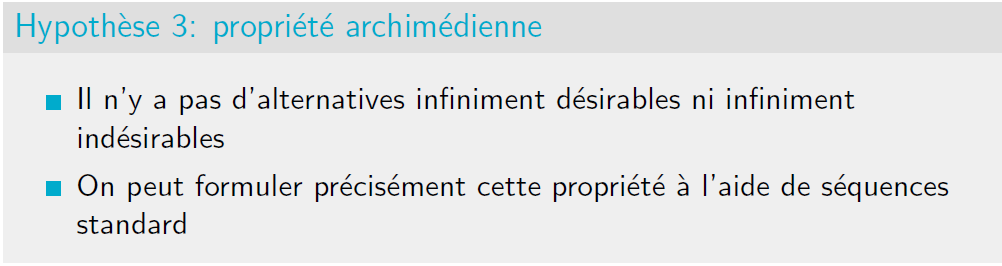
\includegraphics[width=4.5in]{Images/archimedienne}
			\end{center}
			%
		%
		\pagebreak
		%
		\subsubsection{Méthode des échanges égaux}
			\alinea Le but de cette méthode est d'\hl{éliminer les alternatives dominées} et de \hl{supprimer des critères en
				compensant par d'autres critères}. Prenons par exemple les alternatives suivantes (2 critères sont à minimiser, les
				autres à maximiser), on peut retirer \textit{e} car est dominée par \textit{b} et \textit{a} est presque 
				dominée par \textit{d}, on peut donc retirer \textit{a} et \textit{e}. Ensuite, on va chercher à supprimer 
				un critère, et celui qui a le plus de valeur en commun est \textit{Accès}. On va donc chercher à compenser
				le gain en \textit{Accès} par un gain en \textit{Clients}. Pour trouver $\delta$, on demande au décideur 
				pour quel gain en \textit{Clients}, \textit{c} et \textit{c'} seront équivalent à ses yeux.
				Une fois qu'on a déterminé cette valeur, on remplace \textit{c} par \textit{c'} et on supprime le critère
				\textit{Accès} dont toutes les valeurs sont égales.
			%
			\begin{center}
				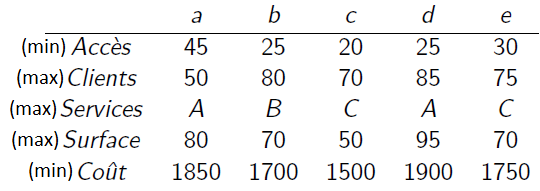
\includegraphics[width=3in]{Images/even_swaps1} 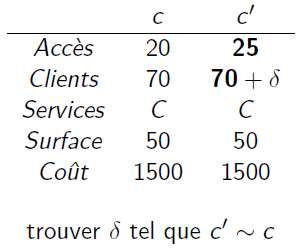
\includegraphics[width=1.5in]{Images/even_swaps2}
				 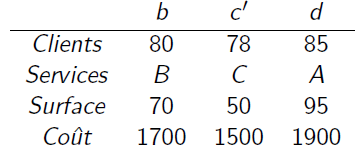
\includegraphics[width=2in]{Images/even_swaps3}
			\end{center}
			%
			\alinea On recommence le procédé ((1) chercher les dominances et retirer les alternatives dominées et (2) supprimer
				des critères en compensant par d'autres critères) jusqu'à n'avoir qu'une seule possibilité restante.
				Cependant : 
			%
			\begin{center}
				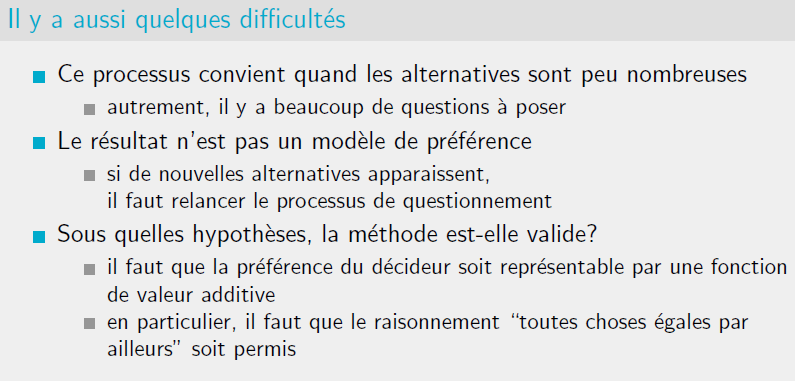
\includegraphics[width=4.5in]{Images/even_swaps4}
			\end{center}
			%
		%
	%
%
\section{Méthode de Saaty (AHP)}
	\alinea Le principe de cette méthode est d'effectuer des comparaisons par paires. Soit par paires d'alternatives, auquel cas
		on obtient un classement au bout de la méthode, soit par paires de critère, ce qui permet d'évaluer le poids de chaque 
		critère. La comparaison par paire (pour un critère $i$ dans le cas d'une alternative) va donner une matrice $\alpha_i$. 
		Une case $\alpha_i (a, b)$ de cette matrice veut dire que l'alternative (ou le critère) \hl{$a$ est $\alpha_i (a, b)$ 
		plus important que $b$ dans la décision finale}. Dans le cas d'une comparaison entre alternatives, on a alors que
		$$\hl{ }\alpha_i (a, b) \approx \frac{u_i(a)}{u_i(b)}\hl{ }$$ et dans le cas d'une comparaison de critères, on a que
		$$\hl{ }\alpha (\text{crit}_1, \text{crit}_2) \approx \frac{k1}{k2} \hl{ }$$
	%
	~\\
	%
	\alinea Une telle matrice est \hl{réciproque}, c'est-à-dire que $ \alpha_i (a, b) = \frac{1}{\alpha_i (b, a)} $. On dit qu'elle
		est parfaitement \red{cohérente} si $\forall a,b,c : \alpha_i (a, b) = \alpha_i (a, c) \cdot \alpha_i (c, b)$.
		A partir de cette matrice, on peut estimer $u_i(a), \forall a$. Pour ce faire, on peut utiliser la \red{méthode des moindres
		carrés}, ou alors on peut utiliser la méthode des vecteurs propres expliquée ci-dessous.
	%
	\subsection{Vecteurs propres}
		\alinea Cette méthode des \red{vecteurs propres} approxime $u_i$ par le vecteur propre normalisé $w_i$.
			La composante (de ligne) $w_i (a)$ de $w_i$ vaut : 
			$$ w_i (a) = \lim\limits_{k \rightarrow \infty} \frac{\alpha_i^k (a, b)}{\sum\limits_{c} \alpha_i^k(c, b)} $$
			On a donc que $w_i$ est approximé par une colonne de la k$^{\text{ème}}$ puissance de la matrice $\alpha_i$, normalisé
			par la somme des éléments de cette colonne. C'est aussi vrai pour la \hl{somme des colonnes, normalisée, de la puissance de la
			matrice}\\
		%
		~\\
		%
		\alinea \hl{Avec $k = 2$, on a déjà une bonne approximation} !  Voici les \hl{étapes} pour calculer l'approximation de $u_i$ 
			en cas de comparaison d'alternatives, ou des poids $k$ en cas de comparaison de critères :
			\begin{enumerate}
				\setlength\itemsep{0cm}
				\item Prendre le carré de la matrice de comparaison par paire.
				\item Sommer les lignes de cette nouvelles matrice, et normaliser ces sommes afin qu'elles somment à 1.
				\item Recommencer à l'étape 1 en utilisant la matrice carrée comme entrée dans le cas ou la différence
					entre le vecteur calculé à cette étape et le vecteur précédente est insignifiante.
			\end{enumerate}
		%
		Voici une illustration de l'étape 2 : 
		\begin{center}
			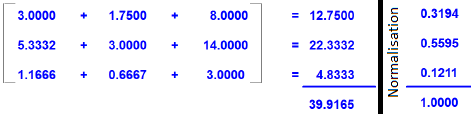
\includegraphics[width=4.5in]{Images/ahp}
		\end{center}
		%
	%
	\begin{center}
		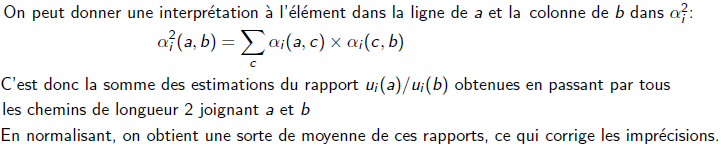
\includegraphics[width=\textwidth]{Images/ahp2}
	\end{center}
	%
	\subsection{Profondeur d'arbre}
		\alinea Tout ceci est valable pour un arbre à trois niveaux : But, Critères, Alternatives. Cependant, il pourrait
			y avoir plus de niveaux (sous-critères).
			\begin{center}
				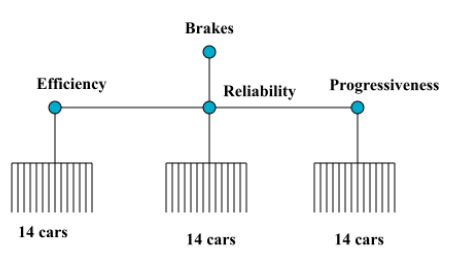
\includegraphics[width=3in]{Images/ahp3}
			\end{center}
	%
	\begin{center}
		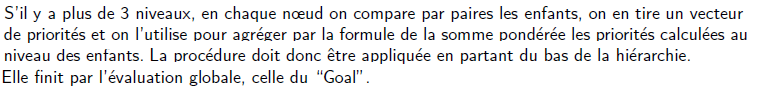
\includegraphics[width=\textwidth]{Images/ahp4}
	\end{center}
	%
	\subsection{\'Evaluations verbales}
		\alinea Pour établir les comparaisons par paires, on pourrait faire appel à une évaluation verbale : Bon, moins bon, etc...
			Cependant, on doit ensuite procéder à un re-codage de ces termes en nombres. Et selon l'échelle choisie, les résultats seront
			très différents. \hl{Il ne faut pas utiliser les comparaisons verbales en pratique. Mieux vaut utiliser une échelle fixée.}
		%
	%
	\subsection{Critique de l'AHP}
		\begin{center}
			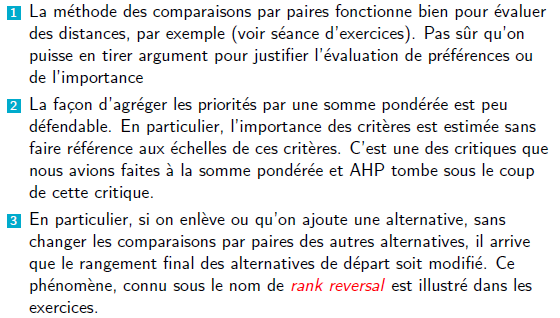
\includegraphics[width=5in]{Images/ahp5}
		\end{center}
	%
%
\section{Surclassement}
	\alinea On dit que l'alternative $a$ \red{\hl{surclasse}} l'alternative $b$
	\begin{itemize}
		\setlength\itemsep{0cm}
		\item Si l'ensemble des critères sur lesquels $a$ est meilleure que $b$ est suffisamment important (\red{concordance}). 
			(Possibilité de faire des coalitions de critères et de poser des conditions sur les critères à prendre).
			En pratique on accorde des poids (qui somment à 1) à chaque critère, et il faut que la \hl{somme des poids des critères où $a$
			est meilleur que $b$ dépasse le seuil $\lambda$}. \hl{Ces poids ne sont pas des taux de substitution}.
		\item Sans que $a$ soit inacceptablement moins bonne que $b$ sur un critère (\red{veto}).
	\end{itemize}
	%
	\begin{center}
		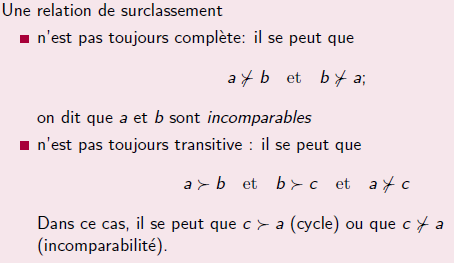
\includegraphics[width=4in]{Images/surclassement}
	\end{center}
	%
	\subsection{Procédures de vote}
		\alinea En utilisant le vote, on va montrer qu'\hl{il n'existe pas de procédure idéale pour la comparaison par paire}.
		%
		\subsubsection{Vote par majorité simple}
			\alinea C'est le vote le plus simple : on demande aux gens de \hl{voter pour leur favoris}, celui qui obtient la majorité
				gagne. Cependant, \hl{le résultat peut ne pas contenter la majorité des personnes} (dû à leur préférences secondaires).
			%
		%
		\subsubsection{Vote par agenda}
			\alinea Les votes par agenda sont très sensibles à leur "agenda". Un agenda est un ordre dans lequel on effectue un vote. 
				Les exemples suivant ont été construit avec les même votant (et donc les même préférences). Selon l'ordre
				dans lequel on effectue le vote (d'abord E-C puis E-R, ou C-R puis C-E), le résultat diffère.
			%
			\begin{center}
				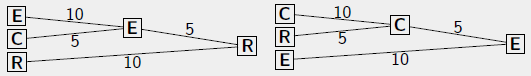
\includegraphics[width=4.5in]{Images/agenda}
			\end{center}
			%
		%
		\subsubsection{Vote en deux tours}
			\alinea Procédure où le premier tour sert à \hl{se concentrer sur deux candidats uniquement}. Les votes qui allaient 
				aux candidats éliminés reviennent à la deuxième préférence de ces votants (selon les candidats restants).
				Le problème est que \hl{cette procédure de vote est non-séparable}. On ne peut pas effectuer ça par région, car le 
				résultat du premier tour pourrait différer selon les zones.
			%
		%
		\subsubsection{Vote par score (Borda)}
			\alinea On donne un score entre $1$ et $X$ pour ses $X$ premières préférences. Ensuite, \hl{le total des scores obtenu pour 
				chaque candidat détermine le vainqueur}. Le problème d'une telle procédure est que les partisans des candidats pourraient
				\hl{tenter de pénaliser un concurrent direct en le classant dernier}, et les résultats sont au final biaisés de 
				cette manière.
			%
		%
		\subsubsection{Vote par circonscription}
			\alinea S'il faut obtenir une majorité de voix dans la majorité des circonscriptions, on peut gagner l'élection avec
				26\% des voix globales car la taille des circonscriptions diffère.
			%
		%
		\subsubsection{Représentation proportionnelle}
			\alinea Si on veut proposer un certain nombre de places pour un certain nombre d'élu, une approche proportionnelle
				par la règle du plus grand reste donne des résultats peu logiques...
			%
			\begin{center}
				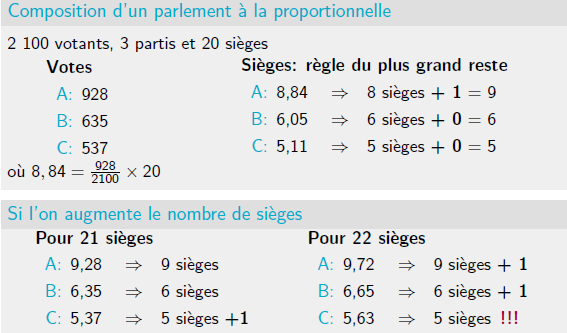
\includegraphics[width=4.5in]{Images/proportions}
			\end{center}
			%
		%
		\subsubsection{Coalitions}
			\alinea Le poids d'un parti n'est pas égal à son nombre de siège ou d'actions. 
			%
			\begin{center}
				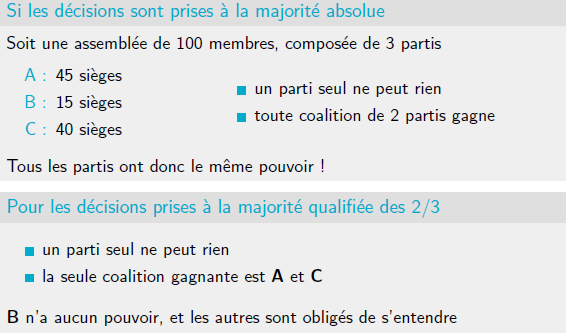
\includegraphics[width=4.5in]{Images/coalitions}
			\end{center}
			%
		%
		\subsubsection{Théorème d'Arrow}
			\begin{center}
				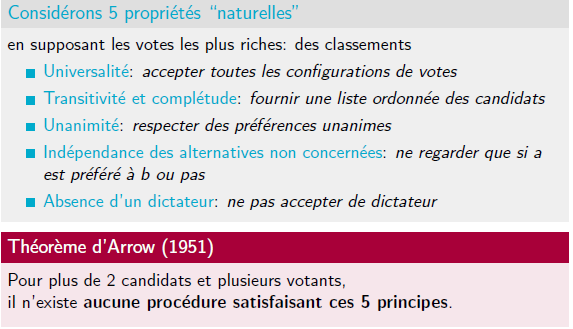
\includegraphics[width=5in]{Images/arrow}
			\end{center}
			%
			\alinea Par exemple, le problème de la technique de Borda est qu'elle ne respecte pas l'indépendance des alternatives 
				non-concernées. Si un candidat mal placé se retire, il se peut que l'ordre des candidats restant change.
			%
		%
		\subsubsection{Théorème de Gibbard et Satterthwaite}
			\begin{center}
				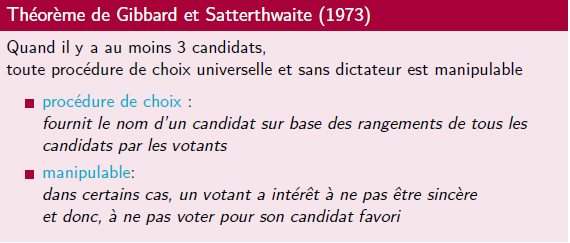
\includegraphics[width=5in]{Images/gibbard}
			\end{center}
			%
		%
	%
	\subsection{Ranger selon des comparaisons par paires}
		\alinea Par défaut, une relation de surclassement vérifie toutes les propriétés du théorème d'Arrow, \hl{sauf la 
			transitivité et complétude}. Il faut donc retravailler le surclassement afin de trouver un rangement à partir
			de celle-ci. \c Ca s'appelle la \red{\hl{phase d'exploitation}}. Voici un exemple de matrice de surclassement.
			Une case $(i, j)$ de la matrice valant 1 signifie que l'alternative $i$ \hl{surclasse} l'alternative $j$.
			On peut voir qu'il existe un cycle de surclassement, et que le tableau ne respecte donc pas toutes les propriétés
			d'Arrow.
		%
		\begin{center}
			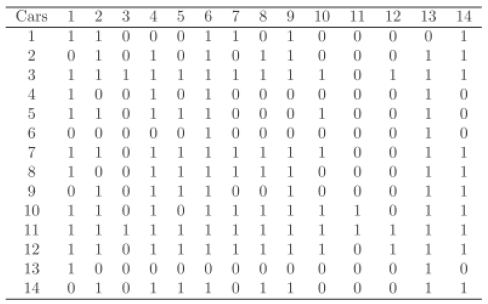
\includegraphics[width=4in]{Images/surclassement2}
		\end{center}	
		%
		\alinea Plusieurs méthodes existent pour la phase d'exploitation.
		%
		\subsubsection{Sommes simples}
			\alinea On peut soit \hl{sommer les lignes}, auquel cas le meilleur est le maximum ou \hl{sommer les colonnes}, auquel cas
				le meilleur est le minimum.
			%
		%
		\subsubsection{ELECTRE}
			\paragraph{ELECTRE I}
				\begin{center}
					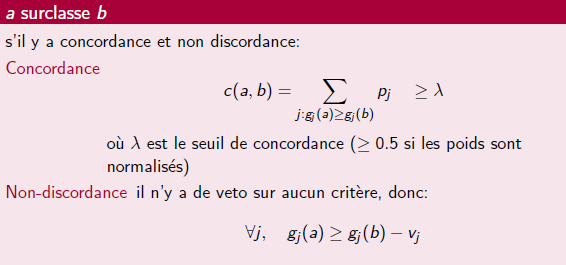
\includegraphics[width=4.5in]{Images/electre_1}
				\end{center}
				%
			%
			\paragraph{ELECTRE II}
				\begin{center}
					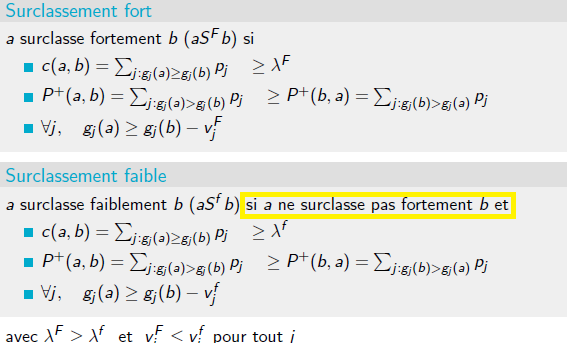
\includegraphics[width=4.5in]{Images/electre_2}
				\end{center}
				%
				\subparagraph{Distillation}
					\alinea Processus itératif qui vise à retirer les circuits. A chaque itération, on retire de la matrice 
						(et on attribue une	place) l'alternative (ou les alternatives en cas d'égalité) qui est surclassée
						par le moins d'autres alternatives (\hl{qui est battue par le moins de monde}). On retire
						donc \hl{du meilleur au moins bon}.
					%
				%
				\subparagraph{Décantation}
					\alinea Processus itératif qui vise à retirer les circuits. A chaque itération, on retire de la matrice 
						(et on attribue une	place) l'alternative (ou les alternatives en cas d'égalité) qui surclasse le moins
						d'autres alternatives (\hl{qui bat le moins de monde}). On retire donc \hl{du moins bon au meilleur}.
					%
				%	
				\subparagraph{Rangement moyen}
					\alinea Le principe est d'appliquer \hl{une distillation, une décantation et de sommer le rang} obtenu par les 
						alternatives lors de ces deux procédures. Après normalisation, on obtient un rangement des alternatives.
					%
				%			
			%
		%		
	%
	\subsection{Fonctions de valeur additive VS surclassement}
		\begin{center}
			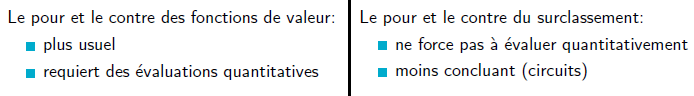
\includegraphics[width=6in]{Images/fva_vs_surclassement}
		\end{center}
	%
%
\section{Méthodes de tri}
	\subsection{Ranger VS trier}
		\begin{center}
			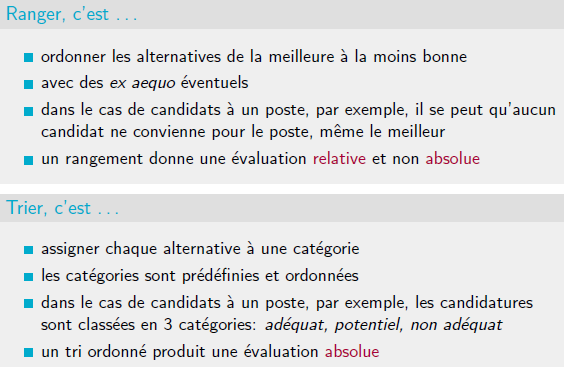
\includegraphics[width=5in]{Images/ranger_vs_trier}
		\end{center}
		%
		\begin{center}
			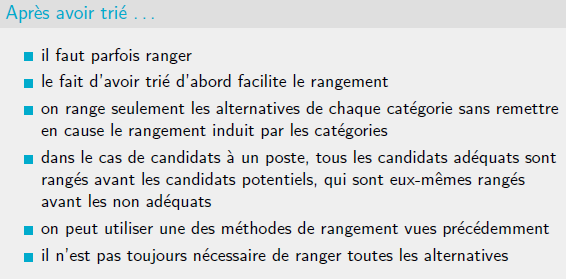
\includegraphics[width=5in]{Images/trier}
		\end{center}
		%
	%
	\subsection{Fonction de valeur}
		\alinea On peut utiliser des \hl{fonctions de valeurs avec des seuils}. Par exemple, si l'alternative dépasse le seuil,
			on le met dans la catégorie A, et sinon dans la catégorie B.\\
		%
		~\\
		%
		\alinea Ces fonctions de valeurs et ces seuils peuvent s'apprendre de manière automatisée par la méthode UTA.
		%
	%
	\subsection{Surclassement}
		\begin{center}
			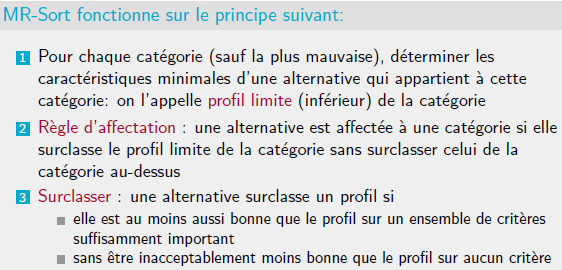
\includegraphics[width=5in]{Images/mr_sort}
		\end{center}
		%
		\begin{center}
			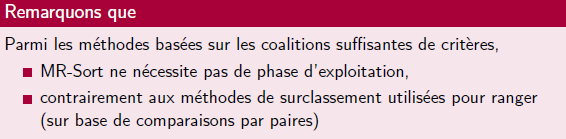
\includegraphics[width=5in]{Images/mr_sort_note}
		\end{center}
		%
	%
%
\section{Décision dans le risque et l'incertain}
	\subsection{Décision dans l'incertain}
		\begin{center}
			
\includegraphics[width=6in]{Images/incertain}
		\end{center}
		%
		\alinea Le principe pour résoudre ce genre d'exercice est de \hl{calculer les probabilités}, et ensuite de \hl{calculer
			l'espérance de gain pour chaque action considérée}.
		%
		\paragraph{Exemple} Illustrons par un exemple :
			%
			\begin{center}
				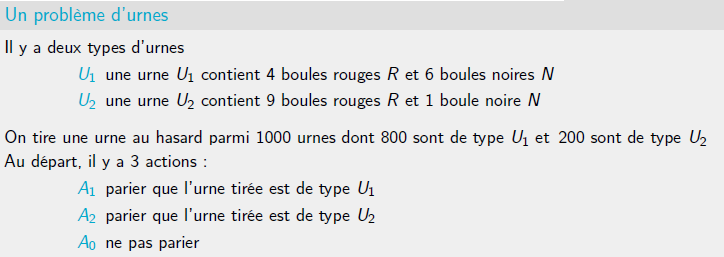
\includegraphics[width=6in]{Images/urnes}
			\end{center}
			%
			\begin{minipage}{0.6\textwidth}
				On remarque qu'en sommant le nombre total de boules rouges, et en sommant le nombre total de boules noires, il y en
					a 5000 de chaque sorte : \#R = $(800 \cdot 4 + 200 \cdot 9) = 5000$, et \#N = $(800 \cdot 6 + 200 \cdot 1) = 5000$.
			\end{minipage}\hfill
			\begin{minipage}{0.33\textwidth}
				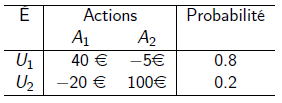
\includegraphics[width=\textwidth]{Images/urnes3}
			\end{minipage}~\\~\\~\\
			%
			De plus, imaginons que l'on puisse payer pour obtenir des informations. L'exemple prendra l'\hl{action d'information} 
				$e_1$ qui consiste à tirer au hasard une boule de l'urne choisie pour 8 euros. Pour calculer les probabilités des 
				résultats d'une telle action, il faut utiliser la théorie probabiliste suivante :
			%
			\begin{center}
				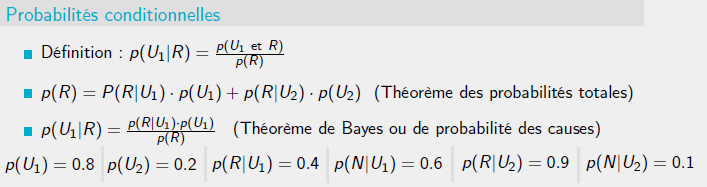
\includegraphics[width=6in]{Images/proba}
			\end{center}
			%
			\begin{center}
				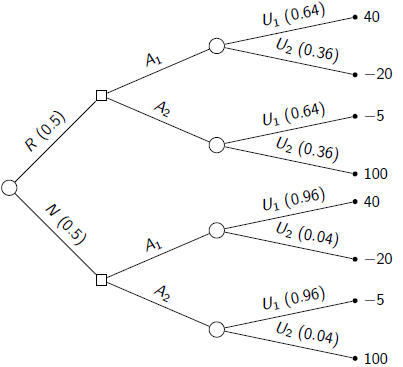
\includegraphics[width=3in]{Images/urnes4}
			\end{center}
			%
			Ensuite, pour calculer l'espérance de gain, on va partir des feuilles de l'arbre, et \hl{calculer le gain moyen 
				pour chaque action}, en comptant les probabilités calculées précédemment.
			%
			\begin{center}
				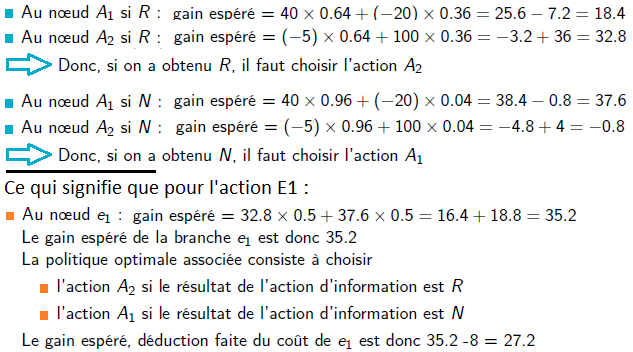
\includegraphics[width=5.5in]{Images/urnes2}
			\end{center}
			%
		%
	%
	\subsection{Décision dans le risque}
		\alinea \hl{L'espérance n'est pas une mesure qui représente au mieux le choix du décideur} lorsque celui peut y perdre.
			En effet, les loteries suivantes ont la même espérance, mais il peut paraître très risqué de pouvoir perdre 
			le montant d'argent de la loterie B.
		%
		\begin{center}
			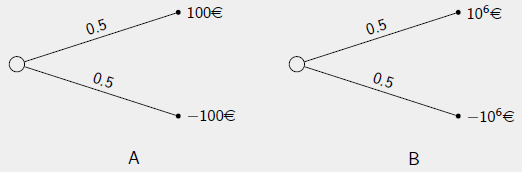
\includegraphics[width=3in]{Images/loteries}
		\end{center}
		%
		\subsubsection{Espérance-Variance}
			Une première idée est de rajouter la variance dans le calcul, cependant, là encore, il peut y avoir des choix ambigus.
			%
			\begin{center}
				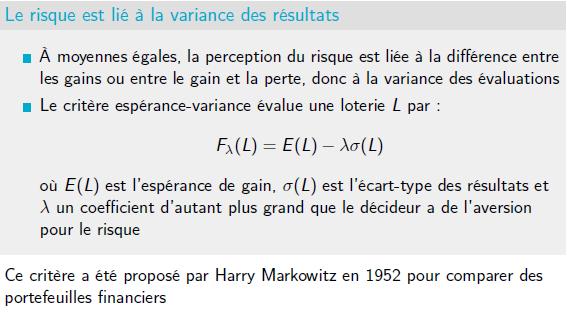
\includegraphics[width=4.5in]{Images/markowitz}
			\end{center}
			%
			\hl{Rappel :} \\
			%
			\begin{minipage}{0.24\textwidth}
				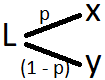
\includegraphics[width=0.5\textwidth]{Images/loteries3}
			\end{minipage}\hfill
			\begin{minipage}{0.75\textwidth}
				$ E(L) = p\cdot x + (1 - p) \cdot y $ ~\\
				$ \sigma(L) = \sqrt{p \cdot (x - E(L))^2 + (1 - p) \cdot (y - E(L))^2} $
			\end{minipage}~\\~\\~\\
			%
			Les loteries suivantes ont le même critère espérance-variance.
			%
			\begin{center}
				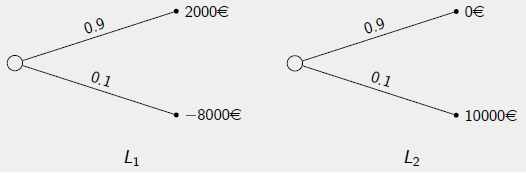
\includegraphics[width=3in]{Images/loteries2}
			\end{center}
			%
		%
		\subsubsection{Utilité espérée}
			\begin{minipage}{0.66\textwidth}
				\alinea L'utilité espérée va dépendre de l'\hl{aversion au risque du décideur}. Celle-ci s'évalue en posant des questions.
				Les questions sont du style à proposer des valeurs pour $x$ au décideur pour qu'il trouve L1 équivalent à L2. 
				On va proposer alternativement des valeurs hautes et des valeurs basses afin de trianguler le prix idéal pour le décideur.
			%
			\end{minipage}\hfill
			\begin{minipage}{0.3\textwidth}
				\includegraphics[width=\textwidth]{Images/aversion}
			\end{minipage}~\\~\\~\\
			%
			Une fois qu'on a trouvé $x$, \hl{on place $x$ à 0.5 de la fonction d'utilité}. On va \hl{chercher des valeurs intermédiaires}. 
				On va donc reposer la même question, mais cette fois ci en fixant les valeurs de L1 entre  0 et $x$ et ensuite entre $x$ 
				et 10000. On répète ainsi de suite jusqu'à avoir le degrés de précision recherché.
			%
			\paragraph{Von Neumann et Morgenstern}~\\~\\
				\alinea Cette technique est réalisable si la comparaison entre loterie respecte 5 axiomes amenés par 
					\hl{Von Neumann et Morgenstern} : 
				%
				\begin{center}
					\includegraphics[width=\textwidth]{Images/von_neumann-morgenstern}
				\end{center}
				%
				\begin{center}
					\includegraphics[width=\textwidth]{Images/von_neumann-morgenstern2}
				\end{center}
			\paragraph{Aversion VS Goût}~\\~\\
				\begin{minipage}{0.6\textwidth}
					\alinea On notera alors qu'une fonction d'utilité \red{concave} (gauche) représente une 
					\hl{aversion pour le risque} tandis 
					qu'une fonction d'utilité \red{convexe} (droite) représente un \hl{goût pour le risque}. Une attitude \red{neutre} 
					se traduit alors par une fonction d'utilité \hl{linéaire}. Le décideur peut toujours changer de comportement au cours 
					de la fonction d'utilité (point d'inflexion).
				\end{minipage}\hfill
				\begin{minipage}{0.33\textwidth}
					\includegraphics[width=\textwidth]{Images/aversion_gout}
				\end{minipage}~\\~\\~\\
				%
				\alinea La façon de poser la question au décideur influencera son aversion ou son goût pour le risque. En effet,
					le décideur doit se baser sur \hl{un point de référence} qui peut être le gain/perte ou la modification de 
					son capital (10000 => 10050 ou 10000 => 9950).
				%
			%
			\paragraph{\'Evaluation du risque} ~\\~\\
				\alinea On dira en général qu'un risque s'évalue selon sa fréquence $\times$ sa gravité
				%
				\begin{center}
					\includegraphics[width=4.5in]{Images/evaluation_risque}
				\end{center}
				%
			%
		%
	%
%
\section{Optimisation Multi-Objectif}
	\alinea Le plus simple est d'expliquer la résolution sur un exemple de minimisation. Si jamais \hl{on a une maximisation, on doit 
		repasser en minimisation} ! La représentation du milieu contient les solutions admissibles.
		La représentation toute à droite est l'\red{espace des critères}, et regroupe 
		l'\hl{image de l'ensemble des solutions admissibles}. Pour passer de l'un à l'autre, on prend les coins (ou plus généralement :
		les points) et on les représente selon leur images en fonction des critères. Deux points ont été liés, on pourrait 
		faire de même avec les deux autres...~\\
	%
	\begin{minipage}{0.25\textwidth}
		\includegraphics[width=\textwidth]{Images/multi-obj}
	\end{minipage}\hfill
	\begin{minipage}{0.66\textwidth}
		\includegraphics[width=\textwidth]{Images/decisions}
	\end{minipage}~\\~\\~\\
	%
	\alinea Pour choisir une solution, on va avoir recours à une comparaison de vecteurs.
	%
	\begin{center}
		\includegraphics[width=\textwidth]{Images/dominance}
	\end{center}
	%
	\alinea Par cette notion de dominance, on peut trouver le front de Pareto de notre exemple.
	%
	\begin{center}
		\includegraphics[width=5in]{Images/pareto}
	\end{center}
	%
	\alinea En général, voilà \hl{les différences entre les sortes de dominances} :
	%
	\begin{center}
		\includegraphics[width=0.95\textwidth]{Images/efficace}
	\end{center}
	%
	\subsection{Points spéciaux}
		\alinea On peut distinguer trois points spéciaux : le point idéal ($y^I$), le point anti-idéal ($y^{AI}$) et le 
			point Nadir ($y^N$).~\\~\\
		%
			\begin{minipage}{0.8\textwidth}
				\includegraphics[width=5in]{Images/points}
			\end{minipage}\hfill
			\begin{minipage}{0.19\textwidth}
				\hl{On a} $ \forall y \in Y_N:  $
				$$ y_k^{I} \leqslant y_k $$
				$$ y_k \leqslant y_k^N $$
			\end{minipage}
		%
	%
	\subsection{Optimum lexicographique}
		$$ y1 <_{lex} y2 \text{\ \ \ si\ \ \ } y1_q < y2_q \text{\ \ \ où\ \ \ } q = \min\{k: y1_k \neq y2_k\} $$
		%
		\alinea Autrement dit, on doit penser comme l'ordre alphabétique : on regarde 'lettre' par 'lettre' jusqu'à tomber sur une
			différence, et puis on compare cette lettre : $ (2, 3, 4) <_{lex} (2, 3, 5) $. On peut éventuellement \hl{ranger les
			dimensions (critères) des solutions par ordre d'importance} ! Une solution $x$ est un \red{optimum lexicographique}
			si $\forall x': f(x) <_{lex} f(x') $. \\ \hl{optimum lexicographique $\Rightarrow$ solution efficace}.
		%
	%
	\subsection{Résolution d'un problème}
		\alinea On a besoin des contraintes suivantes :
		%
		\begin{itemize}
			\setlength\itemsep{0cm}
			\item $X_E \neq \emptyset$
			\item $y^I \neq y^N$
		\end{itemize}
		%
		\alinea Notre méthode doit être \red{correcte} (les solution trouvées sont efficaces) et \red{complète} 
			(on trouve toutes les solution efficaces). Pour ce faire, on peut faire une somme pondérée des critères
			avec un paramètre $\lambda$ qui est un vecteur de poids :
			$$ sol = \min \lbrace \sum\limits^p_{k=1} \lambda_k f_k(x) : x \in X \rbrace\text{, avec } \lambda \succ 0 $$
			$ \lambda \succ 0 $ signifie qu'au moins une des composantes de lambda doit être supérieure à $0$.
		%
		\begin{center}
			\includegraphics[width=5.5in]{Images/lambda}
		\end{center}
		%
		\alinea On peut prouver qu'une \hl{solution optimale} de la formule ci-dessus est \hl{faiblement efficace}. Si la solution optimale
			est \hl{unique}, alors elle est \hl{efficace tout court}. De plus, si une solution est \hl{optimale avec $\lambda > 0$}
			(toutes les composantes $>$ 0), alors \hl{la solution est efficace (qu'elle soit unique ou non)}.
		%
		\paragraph{\hl{Théorème de Geoffrion} (sol. correctes)} Si $Y = f(X)$ est \red{convexe}, alors si $x$ est faiblement efficace, 
			$\exists \lambda \succ 0$ t.q. $x$ est solution optimale de $\min \lbrace \sum\limits^p_{k=1} \lambda_k f_k(x) : 
			x \in X \rbrace$. (Rappel: un polygone est convexe si n'importe quelle ligne tracée en son sein est entièrement comprise
			dans le polygone. Ce n'est pas le cas des exemple plus haut.)\\
			Dans le cas \hl{non-convexe}, les solutions efficaces \red{supportées} sont les solution efficaces $x$ telles que $f(x)$ 	
			appartiennent à l'\hl{enveloppe convexe} du polygone.
		%
		\begin{center}
			\includegraphics[width=4.5in]{Images/convexe}
		\end{center}
		%
		\paragraph{\hl{Compromis}} Le principe est de trouver un point à une distance minimale du point idéal.
			\begin{center}
				\includegraphics[width=4.5in]{Images/distance}
			\end{center}
		%
	%
	\subsection{Préférences du décideur}
		\alinea Le principe est de construire une \hl{fonction d'utilité pour chaque critère} afin de "pondérer" les solutions trouvées.
			On peut également lui proposer des solutions afin qu'il donne un avis sur le résultat selon chaque critère.
		%
		\paragraph{Méthode de Steuer and Choo} Cette méthode peut s'appliquer à des problèmes non linéaires. Le principe
			est de donner des solutions efficaces (calculée grâce à une distance d'un point idéal ou utopique) au décideur et de lui
			demander laquelle il préfère. On recommence ensuite avec des poids et des distances proches de la solution choisie 
			précédemment. Une fois que le décideur est satisfait, on peut s'arrêter.
		%
	%
	\pagebreak
	%
	\subsection{Optimisation combinatoire (discrète) multi-objectifs}
		\alinea Le principe est ici de fonctionner avec l'enveloppe convexe des solutions: 
			\begin{center}
				\includegraphics[width=5in]{Images/combinatoire}
			\end{center}
		%
		\alinea Les solutions à l'intérieur de cette enveloppe sont considérés comme "non-supportés".
		%
		\begin{center}
			\includegraphics[width=3.5in]{Images/combinatoire2}
		\end{center}
		%
	%
%
\pagebreak
%
\section{Théorie des jeux}
	\alinea Dans la théorie des jeux, on a des joueurs et des actions que ces joueurs peuvent effectuer.
	%
	\subsection{Vocabulaire}
		\begin{center}
			\includegraphics[width=5in]{Images/cooperatif}
		\end{center}
		%
		\begin{center}
			\includegraphics[width=3.25in]{Images/simultane_sequentiel}
		\end{center}
		%
		\begin{center}
			\includegraphics[width=4in]{Images/symetrique}
		\end{center}
		%
		\begin{center}
			\includegraphics[width=4.5in]{Images/repete}
		\end{center}
		%
		\begin{center}
			\includegraphics[width=6in]{Images/itere}
		\end{center}
		%
		\begin{itemize}
			\setlength\itemsep{0cm}
			\item \red{Stratégie pure} : choisir une action parmi celles proposées.
			\item \red{Stratégie mixte} : choisir une action \hl{selon des probabilités} (e.g. on lance un dés pour déterminer quelle 
				action jouer...).
			\item \red{\'Equilibre de Nash} : paire de stratégie de laquelle aucun des deux joueurs n'a un intérêt personnel à changer
				unilatéralement de stratégie.
			\item \red{Jeux de coordination} : les joueurs ont intérêt à adopter tous les deux la même action.
			\item \red{Jeux d'anti-coordination} : les joueurs ont intérêt à adopter des actions différentes.
		\end{itemize}
		%
	%
	\subsection{Dominance}
		\alinea On peut appliquer le principe de dominance par ligne ou par colonne. Prenons comme un exemple un 
			\red{dilemme du prisonnier} (à minimiser) (à gauche : un exemple; à droite : la formule générale) : 
		%
		\begin{center}
			\includegraphics[width=2.5in]{Images/prisonnier} \hfill \includegraphics[width=3.25in]{Images/prisonnier2}
		\end{center}
		%
		\alinea Sur l'exemple, la ligne entourée domine la ligne non-entourée pour le joueur Lig (Scores : 10 < 20 et 1 < 2),
			et la colonne entourée domine la colonne non-entourée pour le joueur Col (Scores : 10 < 20 et 1 < 2). L'intersection
			est alors (10, 10) ce qui représente un assez mauvais score pour les deux joueurs... Le plus logique aurait été
			(2, 2) qui est un assez bon score pour les deux joueurs => \hl{Dans un dilemme du prisonnier, la dominance conduit à un
			résultat sous-optimum.}\\
		%
		~\\
		%
		\alinea \hl{Dans un jeu séquentiel}, la dominance se calcule selon un principe de récursion arrière (on part de la fin pour arriver
			au début, toujours en prenant l'action qui nous intéresse le plus ce tour-ci).\\
		%
		~\\
		%
		\alinea Dans un jeu à $n$ joueurs, le principe reste le même. Prenons 3 comme exemple. 3 joueurs ont chacun deux actions 
			possible : 
			\begin{itemize}
				\setlength\itemsep{0cm}
				\item J1 -- A, B
				\item J2 -- F, G
				\item J3 -- X, Y
			\end{itemize}
			Voici la liste des payoffs : 
			\begin{center}
				\begin{tabular}{|c|c|c|c|c|}
					\hline
					\textbf{Actions jouées (J1 J2 J3)} & \textbf{Score J1} & \textbf{Score J2} & \textbf{Score J3} & \textbf{Gardé par}\\
					\hline
					AFX & 1 & 6 & 9 & /\\
					AFY & 2 & 5 & 8 & /\\
					AGX & 3 & 9 & 9 & /\\
					AGY & 4 & 8 & 7 & /\\
					\green{BFX} & 2 & 1 & 3 & J1, J2, J3\\
					BFY & 3 & 2 & 2 & J1, J2\\
					BGX & 4 & 0 & 7 & J1\\
					BGY & 5 & 1 & 2 & J1\\
					\hline
				\end{tabular}
			\end{center}
		%
		\alinea On va alors résonner joueur par joueur \hl{de manière rationnelle} (chaque joueur suppose que les autres joueurs 
			maximisent leur propre score et jouent donc de la même manière que le premier). 
			Le joueur 1 va préférer jouer l'action B car dans tous les cas (quelques soient
			les actions que ses adversaires considèrent), l'action B réussi mieux au joueur 1. Maintenant qu'on sait que le joueur 1
			va choisir l'action B, on va regarder les actions plausibles du joueur 2 en fonction. On préfère choisir le F car
			les cas "BG" sont moint intéressant que les cas "BF" pour le joueur 2. Enfin, il reste au joueur 3 à sélectionner une des 
			deux actions restantes. Il va préférer X car l'action lui rapporte 3 tandis que "BFY" ne lui rapporte que 2.
		%
	%
	\subsection{Minimax}
		\alinea Le critère du \red{minimax} s'applique aux \red{\hl{jeux à somme nulle}}. Ces jeux ont une seule notion de score.
			Ce qui est gagné par un joueur est perdu par l'autre. Le but d'un joueur est donc de maximiser le score et celui
			de l'autre joueur est de minimiser le score.
		%
		\paragraph{\'Equilibre pur}~\\~\\
			\begin{minipage}{0.74\textwidth}
				\alinea On dit alors qu'une \red{\hl{paire de stratégies pures en équilibre}} est une paire qui réalise le 
				résultat maximum de 
				sa colonne et le minimum de sa ligne. Dans l'exemple ci-contre, les entourés sont les maximums de colonne et les encadrés 
				sont les minimum de ligne. Un seul membre fait parti des deux ensembles : c'est l'équilibre selon le critère minimax.
				Il \hl{peut y avoir plusieurs paires de stratégies en équilibre}, mais alors elles se situent soit dans la même ligne, soit
				dans la même colonne. Il se \hl{peut qu'il n'y ait pas d'équilibre}.
			%
			\end{minipage}\hfill
			\begin{minipage}{0.2\textwidth}
				\includegraphics[width=\textwidth]{Images/minimax}
			\end{minipage}
			%
		%
		\paragraph{\'Equilibre mixte}
			\alinea On peut également chercher des \red{\hl{stratégies mixtes en équilibre}}. 
			%
		%
		\paragraph{Théorème du minimax}
			\begin{center}
				\includegraphics[width=4.45in]{Images/minimax_theoreme}
			\end{center}
			%
			\begin{center}
				\includegraphics[width=4.45in]{Images/minimax_preuve}
			\end{center}
			%
		%
	%
	\subsection{\'Equilibre de Nash}
		\alinea Un équilibre de Nash est un équilibre duquel aucun des deux joueurs n'a intérêt à changer unilatéralement d'action.
			Dans l'exemple suivant, les deux équilibres purs sont mis en évidence. Depuis l'équilibre encadré, le joueur $L$ n'a pas
			intérêt à passer de l'action $L_1$ à $L_2$ car il y perdrait 1, et le joueur $C$ n'a pas intérêt à passer de l'action $C_2$
			à $C_1$ car il y perdrait 99.
		%
		\begin{center}
			\includegraphics[width=2.75in]{Images/nash}
		\end{center}
		%
		\alinea Il existe également un équilibre de Nash mixte dans l'exemple ci-dessus. Il se calcule de la manière suivante 
			($EU$ veut dire utilité espérée) :  \\
		%
		~\\
		%
		\ul{Joueur $C$} (on regarde aux actions que peut faire $L$ et au score que ce dernier pourrait obtenir) : \\ 
		$EU(L_1) = -100\cdot p + 1 \cdot (1 - p)$ \\
		$EU(L_2) = -1 \cdot p + 0 \cdot (1 - p)$ \\
		$EU(L_1) = EU(L_2) \text{ (Nash) } \Leftrightarrow -100p + 1 - p = -p \Leftrightarrow p = \frac{1}{100}$\\
		On a donc que le joueur $C$ doit joueur l'action $C_1$ dans $\frac{1}{100}$ des cas, et l'action $C_2$ dans $\frac{99}{100}$ 
			des cas.\\~\\
		%
		\ul{Joueur $L$} (on regarde aux actions que peut faire $C$ et au score que ce dernier pourrait obtenir) : \\ 
		$EU(C_1) = -100\cdot q + 1 \cdot (1 - q)$ \\
		$EU(C_2) = -1 \cdot q + 0 \cdot (1 - q)$ \\
		$EU(C_1) = EU(C_2) \text{ (Nash) } \Leftrightarrow -100p + 1 - q = -q \Leftrightarrow q = \frac{1}{100}$\\
		On a donc que le joueur $L$ doit joueur l'action $L_1$ dans $\frac{1}{100}$ des cas, et l'action $L_2$ dans $\frac{99}{100}$ 
			des cas.
		%
	%
	\subsection{Solution de Nash}
		\alinea Dans un jeu en coopération, les joueurs ont intérêt à trouver un équilibre, sans quoi leur score pourrait être
			mauvais. Dés lors, une solution de Nash peut être trouvée en utilisant des fonctions d'utilité.
		%
		\begin{center}
			\includegraphics[width=4.5in]{Images/axiomes_nash}
		\end{center}
		%
		\begin{center}
			\includegraphics[width=4.5in]{Images/axiomes_nash2}
		\end{center}
		%
	%
	\subsection{Stratégie évolutionnaire stable}
		\alinea En comparant deux stratégies mixtes, une stratégie mixte est dite \red{évolutionnaire stable} si 
			celle-ci a une espérance d'utilité plus élevée que l'autre stratégie.
		%
	%
%
\end{document}